% Configurazione
\documentclass{article}

\usepackage{titling} % Required for inserting the subtitle
\usepackage{graphicx} % Required for inserting images
\usepackage{tabularx} % Per l'ambiente tabularx (tabelle)
\usepackage{calc} % Sempre per le tabelle
\usepackage[hidelinks]{hyperref} % Per i collegamenti ipertestuali, ad esempio sulla table of contents
\usepackage[italian]{babel} % Per la lingua italiana nelle scritte automatiche
\usepackage[table]{xcolor} % Per colorare il testo e le celle delle tabelle
\usepackage{colortbl} % Per colorare le celle delle tabelle
\usepackage{lipsum} % Per generare lorem ipsum
\usepackage[normalem]{ulem} % Per sottolineare il testo
\usepackage{array} % Per la visualizzazione fluttuante di array di domande e risposte
\usepackage{ragged2e} % Pacchetto necessario per \justifying che giustifica il testo di tabelle
\usepackage{tikz} % Per spostare elementi nel documento in modo facile e veloce
\usepackage[a4paper, top=2.5cm, bottom=2.5cm, left=2.5cm, right=2.5cm]{geometry} % Per i margini della pagina
\usepackage{fancyhdr} % Per l'intestazione e il piè di pagina
\usepackage{amsmath} % Per scrivere formule matematiche, in particolare per il pedice G

\newcommand{\ulhref}[2]{\href{#1}{\uline{#2}}} % Nuovo comando per sottolineare i link
\newcommand{\ulref}[1]{\uline{\ref{#1}}} % Nuovo comando per sottolineare i collegamenti a immagini e tabelle
\setlength{\parindent}{0pt} % Rimuove il rientro automatico dei paragrafi
\usetikzlibrary{calc} % Libreria per il calcolo delle coordinate di TikZ
\pagestyle{fancy} % Stile della pagina, per l'intestazione e il piè di pagina
\renewcommand{\footrulewidth}{0.4pt} % Inserimento della linea orizzontale in basso
\setlength{\headsep}{1.4cm} % Spazio tra l'intestazione e il testo
\definecolor{lightgray}{gray}{0.95} % Definizione del colore grigio chiaro

\graphicspath{ {immagini/} {../../../shared/immagini/} }



% Struttura
\begin{document}

\thispagestyle{plain} % Niente intestazione e piè di pagina


\begin{tikzpicture}[remember picture, overlay]
    % Punto di partenza al centro orizzontale nella metà superiore
    \coordinate (top_center) at ($(current page.north)!0.3!(current page.south)$);

    % UniPD: Logo e descrizione
    \node at (top_center) [anchor=north, xshift=-3cm, yshift=4.85cm] 
        {\includegraphics[width=0.15\textwidth]{Logo Universita di Padova.png}};
    \node at (top_center) [anchor=north, xshift=1.7cm, yshift=4.5cm]
        {\textcolor{red}{\textbf{Università degli Studi di Padova}}};
    \node at (top_center) [anchor=north, xshift=1.7cm, yshift=4cm]
        {\textcolor{red}{Laurea: Informatica}};
    \node at (top_center) [anchor=north, xshift=1.7cm, yshift=3.5cm]
        {\textcolor{red}{Corso: Ingegneria del Software}};
    \node at (top_center) [anchor=north, xshift=1.7cm, yshift=3cm]
        {\textcolor{red}{Anno Accademico: 2024/2025}};

    % SWEg Labs: Logo e descrizione
    \node at (top_center) [anchor=north, xshift=-2.85cm, yshift=1.5cm] 
        {\includegraphics[width=0.16\textwidth]{Logo SWEg.png}};
    \node at (top_center) [anchor=north, xshift=1.7cm, yshift=0.5cm]
        {\textbf{Gruppo: SWEg Labs}};
    \node at (top_center) [anchor=north, xshift=1.7cm, yshift=0cm]
        {Email: \textsf{gruppo.sweg@gmail.com}};
\end{tikzpicture}


\vspace{10cm}

{
\centering
\Huge\bfseries Manuale Utente\par
\vspace{0.5cm}
\Large Versione 1.0.0\par
}

\vspace{2cm}
% Intestazione
\fancyhead[L]{1 \hspace{0.2cm} Informazioni generali} % Testo a sinistra

\pagenumbering{arabic} % Numerazione araba per il contenuto


\section{Informazioni generali}

\begin{itemize}
    \item \textbf{Tipo di riunione}: interna
    \item \textbf{Luogo}: meeting \emph{Discord}\textsubscript{\textit{\textbf{G}}}
    \item \textbf{Data}: 04/11/2024
    \item \textbf{Ora inizio}: 17:30
    \item \textbf{Ora fine}: 18:45
    \item \textbf{Responsabile}: Riccardo Stefani
    \item \textbf{Scriba}: Davide Verzotto
    \item \textbf{Partecipanti}:
    \begin{itemize}
        \item Federica Bolognini
        \item Michael Fantinato
        \item Giacomo Loat
        \item Filippo Righetto
        \item Riccardo Stefani
        \item Davide Verzotto
    \end{itemize}
\end{itemize}


\newpage
% Intestazione
\fancyhead[L]{Registro delle modifiche} % Testo a sinistra
\fancyhead[R]{\includegraphics[width=0.16\textwidth]{sweg_logo_sito_inverted.png}} % Immagine a destra

% Piè di pagina
\fancyfoot[L]{Analisi dei Requisiti}       % Testo a sinistra
\fancyfoot[C]{\thepage}                % Numero di pagina al centro
\fancyfoot[R]{Versione 1.0.0}          % Testo a destra

\pagenumbering{roman} % Numerazione romana per l'indice


\section*{Registro delle modifiche}

\begin{table}[h]
    \centering
    \rowcolors{2}{lightgray}{white}
    \begin{tabular}{|c|c|p{5cm}|p{3cm}|p{3cm}|}
        \hline
        \rowcolor[gray]{0.75}
        \textbf{Versione} & \textbf{Data} & \multicolumn{1}{|c|}{\textbf{Descrizione}} & 
        \multicolumn{1}{|c|}{\textbf{Autore}} & \multicolumn{1}{|c|}{\textbf{Verifica}}\\
        \hline
        1.0.0 & ... & Approvazione del documento & Filippo Righetto & Filippo Righetto\\
        \hline
        ... & ... & Verifica del documento & ... & ...\\
        \hline
        0.2.4 & 10-12-24 & Scrittura del caso d'uso \bulhyperlink{UC2}{UC2} & Giacomo Loat & Michael Fantinato \\
        \hline
        0.2.3 & 09-12-24 & Scrittura del caso d'uso \bulhyperlink{UC1}{UC1} & Federica Bolognini & ... \\
        \hline
        0.2.2 & 09-12-24 & Creazione del template per la trascrizione dei casi d'uso in \S\bulref{sec:casi_uso} & Riccardo Stefani & Federica Bolognini\\
        \hline
        0.2.1 & 08-12-24 & Scrittura dei casi d'uso \bulhyperlink{UC5}{UC5}, \bulhyperlink{UC6}{UC6}, \bulhyperlink{UC11}{UC11} e 
        \bulhyperlink{UC16}{UC16} & Riccardo Stefani & Giacomo Loat\\
        \hline
        0.2.0 & 06-12-24 & Verifica del documento allo stato attuale & Riccardo Stefani & Riccardo Stefani\\
        \hline
        0.1.2 & 18-11-24 & Inizio scrittura sezione \S\bulref{sec:Requisiti} & Filippo Righetto & Davide Verzotto\\
        \hline
        0.1.1 & 10-11-24 & Scrittura della sezione \S\bulref{sec:introduzione} di introduzione e della sezione \S\bulref{sec:descrizione_generale} 
        riguardante la descrizione generale & Filippo Righetto & Riccardo Stefani\\
        \hline
        0.1.0 & 05-11-24 & Creazione del documento & Riccardo Stefani & Giacomo Loat\\
        \hline
    \end{tabular}
    \caption{Registro delle modifiche}
\end{table}

\newpage
% Intestazione
\fancyhead[L]{Indice} % Testo a sinistra
\fancyhead[R]{\includegraphics[width=0.16\textwidth]{sweg_logo_sito_inverted.png}} % Immagine a destra

% Piè di pagina
\fancyfoot[L]{Verbale interno}       % Testo a sinistra
\fancyfoot[C]{\thepage}                % Numero di pagina al centro
\fancyfoot[R]{16/11/24}          % Testo a destra

\pagenumbering{roman} % Numerazione romana per l'indice


\tableofcontents
\newpage
% Intestazione
\fancyhead[L]{Elenchi} % Testo a sinistra

\listoffigures

\listoftables
\newpage

% Intestazione
\fancyhead[L]{1 \hspace{0.2cm} Introduzione} % Testo a sinistra

\pagenumbering{arabic} % Numerazione araba per il contenuto 


\section{Introduzione}
Questo documento è stato redatto con l'intento di offrire una trattazione esaustiva e dettagliata 
dei requisiti e dei casi d'uso individuati dal gruppo \textit{sweg labs} nel corso dello sviluppo
del progetto “BuddyBot”. La raccolta di questi dati è il frutto di un'analisi approfondita
del documento di presentazione del \textit{capitolato\textsubscript{G}}, di intense discussioni interne al gruppo di lavoro, 
nonchè di colloqui attivi con il \textit{proponente\textsubscript{G}}, \textit{Azzurrodigitale}.

L'obiettivo è garantire una comprensione completa ed accurata dei requisiti di progetto,
fornendo una base solida per la pianificazione e l'implementazione delle successive fasi di lavoro.

Nel documento adottiamo la sintassi \textit{UML\textsubscript{G}} al fine di formalizzare la rappresentazione e
renderla comprensibile a tutti i potenziali utenti. In particolare, i casi d'uso seguono una
struttura logica e vengono descritti in dettaglio attraverso i seguenti punti:
\begin{itemize}
    \item \textbf{Nominativo:} includiamo il titolo del \textit{caso d'uso\textsubscript{G}} e un breve commento esplicativo;
    \item \textbf{Attori Principali:} identifichiamo chi sono gli \textit{attori\textsubscript{G}} che eseguono le azioni all’interno 
                del caso d'uso;
    \item \textbf{Precondizioni:} specifichiamo lo stato del programma prima dell'esecuzione del caso d'uso;
    \item \textbf{Postcondizioni:} definiamo lo stato del programma dopo il completamento dello scenario del caso d'uso;
    \item \textbf{\textit{Scenario Principale\textsubscript{G}}:} descriviamo in modo dettagliato le azioni svolte durante
                l'esecuzione del caso d'uso, delineando il percorso seguito tra le condizioni iniziali e irisultati ottenuti;
    \item \textbf{Scenari alternativi:} descriviamo gli scenari che diramano dallo scenario principale o le situazioni nelle quali lo svolgimento delle 
                azioni dello scenario principale siaimpossibilitato dalla comparsa di condizioni di errore;
    \item \textbf{\textit{Sottocasi d'uso\textsubscript{G}}:} in alcune circostanze può essere necessaria la definizione di uno
                o più sottocasi d'uso, che andranno ad utilizzare la stessa struttura dei casi d'uso, e potranno essere 
                identificati mediante un numero progressivo nella forma:
                \begin{center}
                    X.Y
                \end{center}
    dove X `e il caso d'uso da cui derivano e Y un numero progressivo ad identificare il sottocaso.
    \item \textbf{Inclusioni:} descrivono funzionalità in comune fra più casi d'uso;
    \item \textbf{Specializzazioni:} possono essere di due tipologie:
    \begin{enumerate}
        \item di attori, dove i figli condividono tutte le funzionalit`a del padre e in pi`u ne
            possiedono di proprie;
        \item di casi d'uso, dove i figli possono aggiungere funzionalit`a rispetto ai padri o
            modificarne il comportamento.
    \end{enumerate}
\end{itemize}

\subsection{Scopo del prodotto}
Nel corso dell'ultimo anno si è verificato un repentino e significativo mutamento nel panorama
dello sviluppo e nell'implementazione dell'\textit{Intelligenza Artificiale\textsubscript{G}}.
Questa trasformazione ha interessato diverse sfaccettature della tecnologia, e si è verificata con il passaggio da un
ruolo prevalentemente incentrato sull'elaborazione e sulla raccomandazione dei contenuti ad
una fase in cui l'Intelligenza Artificiale assume attivamente la responsabilità di generare
contenuti originali. Questa nuova fase ha visto l'emergere di sistemi in grado di creare non
solo testi, ma anche immagini e tracce audio con un livello di sofisticazione che sfida le
precedenti aspettative. \\
Il capitolato\textsubscript{G} C9, 'BuddyBot,' ha come obiettivo la realizzazione di un assistente virtuale (chatbot) 
capace di raccogliere rapidamente informazioni dalle fonti indicate e di fornirle in risposta a domande poste in 
linguaggio naturale tramite chat.\\
Tale assistente virtuale sarà fruibile attraverso una piccola piattaforma web, dove l'utente potrà interagire con l'IA 
per ottenere le risposte desiderate.

\subsection{Glossario}
Al fine di evitare possibili ambiguità relative al linguaggio utilizzato nei documenti, viene fornito un \textit{Glossario}
(attualmente alla sua versione \textit{1.0.0}), nel quale sono contenute le definizioni di termini complessi o aventi uno 
specifico significato. Tali termini, ove necessario, sono segnati in corsivo e marcati con il simbolo G a pedice
(\textit{esempio Way of Working\textsubscript{G}}).

\subsection{Miglioramenti al documento}
La maturità e i miglioramenti sono aspetti fondamentali nella stesura di un documento.
Questo permette di apportare agevolmente modifiche in base alle esigenze concordate tra i
membri del gruppo e il \textit{proponente\textsubscript{G}} nel corso del tempo. Di conseguenza, questa versione del
documento non pu`o essere considerata definitiva o completa, poichè è soggetta a evoluzioni future.

\subsection{Riferimenti}
\subsubsection{Riferimenti normativi}
\begin{itemize}
    \item \href{https://www.sito2.com}{Norme di Progetto (manca link)}
    \item \href{https://github.com/SWEg-Labs/Documentazione/blob/adea4950d9135916b22ef3af717e955f2c11f975/output/RTB/Documentazione%20esterna/piano_qualifica_v1.0.0.pdf}{Piano di qualifica (v 1.0.0)}
    \item \href{https://www.math.unipd.it/~tullio/IS-1/2024/Progetto/C9.pdf}{Capitolato d'appalto C9 - BuddyBot}
    \item \href{https://www.math.unipd.it/~tullio/IS-1/2024/Dispense/PD1.pdf}{Slide PD1 del corso di Ingegneria del Software - Regolamento del Progetto Didattico}
  \end{itemize}

\subsubsection{Riferimenti informativi}
\begin{itemize}
    \item \href{https://github.com/SWEg-Labs/Documentazione/blob/adea4950d9135916b22ef3af717e955f2c11f975/output/RTB/Documentazione%20esterna/glossario_v1.0.0.pdf}{Glossario (v 1.0.0)}
    \item \href{https://github.com/SWEg-Labs/Documentazione/tree/adea4950d9135916b22ef3af717e955f2c11f975/output/RTB/Documentazione%20interna/Verbali%20interni}{Verbali interni}
    \item \href{https://github.com/SWEg-Labs/Documentazione/tree/adea4950d9135916b22ef3af717e955f2c11f975/output/RTB/Documentazione%20esterna/Verbali%20esterni}{Verbali esterni}
    \item \href{https://www.math.unipd.it/~tullio/IS-1/2024/Dispense/T05.pdf}{Slide T05 del corso di Ingegneria del Software - Analisi dei Requisiti}
    \item \href{https://www.sito3.com}{Diagrammi dei casi d'uso (non ho trovato il documento)}
  \end{itemize}

\newpage
% Intestazione
\fancyhead[L]{2 \hspace{0.2cm} Processi primari} % Testo a sinistra


\section{Processi primari}
\label{sec:processi_primari}
\subsection{Fornitura}
\subsubsection{Descrizione}
Questa sezione riporta tutte le norme, gli strumenti e i metodi che ogni membro del gruppo \emph{SWEg Labs} si impegna a rispettare al fine di preservare al meglio i rapporti con il proponente \emph{AzzurroDigitale}\textsubscript{\textit{\textbf{G}}}.
\subsubsection{Scopo}
Il \emph{processo}\textsubscript{\textit{\textbf{G}}} di fornitura intende occuparsi della gestione dei rapporti con il proponente \emph{AzzurroDigitale} con l’obbiettivo di evitare qualsiasi tipo di ostacolo alla comunicazione ed avere un a buona qualità nella stessa.
\subsubsection{Aspettative}
Durante il rapporto il nostro gruppo desidera mantenere una comunicazione disponibile e con \emph{AzzurroDigitale}, in particolare con i referenti Martina Daniele, Camilla Picello, Nicola Boscaro e Mattia Gottardello, così da poter:
\begin{itemize}
    \item Discutere \emph{requisiti}\textsubscript{\textit{\textbf{G}}} chiave necessari da soddisfare nel prodotto finale;
    \item Stabilire tempistiche di lavoro;
    \item Ricevere \emph{feedback}\textsubscript{\textit{\textbf{G}}} sul lavoro in corso;
    \item Ottenere chiarimenti relativi a dubbi e incomprensioni;
    \item Stabilire i \emph{vincoli}\textsubscript{\textit{\textbf{G}}} riguardanti i processi intermedi.
\end{itemize}
\subsubsection{Fasi della Fornitura}
\label{sec:Fasi della Fornitura}
Il processo di fornitura si articola nelle seguenti fasi:
\begin{itemize}
    \item Avvio;
    \item Preparazione della proposta;
    \item Contrattazione;
    \item Pianificazione;
    \item Realizzazione e controllo;
    \item Revisione e Valutazione;
    \item Consegna e Completamento.
\end{itemize}
\subsubsubsection{Avvio}L'attività consiste nelL'attività di avvio consiste nel primo contatto tra il fornitore e il proponente. Durante questa fase, vengono stabiliti i primi accordi e vengono raccolte le informazioni preliminari necessarie per comprendere le esigenze del proponente.
\subsubsubsection{Preparazione della proposta}L'attività si articola nel compito che prevede la formulazione, da parte del fornitore, di una proposta di fornitura che risponda ai requisiti del proponente. La proposta deve essere chiara e dettagliata, in modo da permettere al proponente di valutarla in modo corretto. La preparazione della proposta avviene tramite la redazione di una lettera di presentazione rivolta ai committenti, corredata da un documento indicante il preventivo dei costi e dei tempi necessari alla realizzazione del prodotto, e da un documento che riporta l'analisi dettagliata dell'opportunità.
\subsubsubsection{Contrattazione}L'attività si articola nel compito che prevede la definizione di un contratto tra fornitore e proponente. Il contratto deve essere chiaro e dettagliato, in modo da permettere ad entrambe le parti di avere un quadro chiaro delle attività da svolgere e dei tempi di realizzazione. La contrattazione avviene tramite l'invio della documentazione redatta nella fase precedente al proponente, e la stipula consiste nell'accettazione della proposta da parte del proponente. Da quel momento varranno i vincoli espressi nel documento di preventivo.
\subsubsubsection{Pianificazione}
L'attività di pianificazione consiste nella definizione delle attività da svolgere per la realizzazione del prodotto. Ciò avviene tramite la redazione della documentazione necessaria, e si articola nei seguenti compiti che il fornitore deve svolgere:
\begin{enumerate}
    \item Vengono definiti i requisiti del progetto, i quali vanno poi raccolti in un documento apposito denominato analisi dei requisiti. Andranno a determinare i test necessari alla verifica e validazione del prodotto finale del progetto;
    \item Viene stabilito e adottato un modello di ciclo di vita del software adeguato alla grandezza, alla complessità e alla portata del progetto;
    \item Devono essere stabiliti, da parte del fornitore, i requisiti necessari alla gestione e verifica del progetto e del prodotto, oltre che alla verifica della loro qualità;
    \item Deve essere sviluppato e documentato il piano di gestione del progetto, basandosi sui requisiti individuati al punto precedente, e deve essere redatta una documentazione per descrivere tale piano. Questa documentazionie si baserà sui seguenti punti:
    \begin{itemize}
        \item Struttura organizzativa del progetto e delle autorità. Sono identificati dei ruoli, con compiti, costi e responsabilità differenti, che i membri del team fornitore dovranno ricoprire lungo tutto il progetto, variando tra essi;
        \item Ambiente tecnico. Devono essere riportati gli strumenti a sostegno della realizzazione dei compiti e delle relative attività come parte dei processi in atto nel progetto;
        \item Scomposizione dei processi e delle attività in task eseguibili, in considerazione del budget, delle risorse e del personale disponibile. Nel piano di progetto, la pianificazione delle risorse deve dar luogo ad unpreventivo dei costi, in termini di tempo e risorse, necessari al completamento del progetto. Le task eseguibili saranno assegnate tramite ticket a singoli membri del gruppo, coordinando il lavoro del team tramite unopportuno framework di project management;
        \item Gestione delle caratteristiche qualitative dei prodotti dei processi. In tal senso, deve essere redatto un documento contenente tali metriche, denominato piano di qualifica;
        \item Accertamento della qualità, con il relativo processo di supporto;
        \item Verifica e validazione, con i relativi processi di supporto;
        \item Revisioni congiunte con il cliente, con il relativo processo di supporto mirato al coinvolgimento costante del proponente nella realizzazione del progetto. Un’opportuna verbalizzazione di tali incontri andrà a documentare il loro effettivo avvenimento;
        \item Gestione dei rischi. Un omonimo capitolo deve essere redatto all’interno del piano di progetto, andando ad individuare tutti i potenziali rischi riscontrabili, stimando occorrenza e pericolosità, e identificando un’azione mitigativa da intraprendere in caso di occorrenza effettiva della problematica;
        \item Mezzi di sostegno alla pianificazione e all’analisi dell’avanzamento effettivo. Per facilitare le operazioni di pianificazione, devono essere prodotti dei diagrammi di Gantt , con cui rappresentare graficamente la dislocazione temporale delle attività, rappresentandone la durata, la sequenzialità e il parallelismo;
\end{itemize}
\subsubsubsection{Realizzazione e controllo}
L'attività di realizzazione e controllo consiste nello sviluppo del prodotto software secondo quanto pianificato e nella verifica continua del lavoro svolto. Questa fase si articola nei seguenti compiti:
\begin{itemize}
    \item Osservazione oculata di ciò che prevede il piano di gestione del progetto sviluppato nell’attività precedente;
    \item Sviluppo del codice sorgente, implementazione delle funzionalità e integrazione dei vari componenti del sistema;
    \item Monitoraggio dello stato di avanzamento in relazione all’utilizzo di risorse, sia in termini di budget che di personale, tramite la realizzazione di consuntivi di periodo, analizzando il discostamento di questi ultimi rispetto le stime preventivate nella fase di pianificazione. A sostegno di tale compito, opportune metriche saranno adottate per costituire i grafici del cruscotto valutativo, o dashboard, presente nel documento denominato piano di qualifica;
    \item Identificazione di problemi con opportune fasi retrospettive, documentando ed analizzando questi momenti, con l’intento di giungere ad una soluzione e ad un miglioramento continuo.
\end{itemize}
\subsubsubsection{Revisione e Valutazione}
L'attività consiste L'attività di revisione e valutazione consiste nel verificare che il prodotto sviluppato sia conforme ai requisiti e alle aspettative del proponente. Questa fase deve rispettare i seguenti criteri:
\begin{itemize}
    \item È nell’interesse del team cercare quanto più il confronto conl’azienda proponente, così da ricevere costantemente feedback sull’operato del gruppo. Il fornitore deve essere parte attiva nella coordinazione delle comunicazioni con l’acquirente;
    \item Il dialogo con il proponente deve essere supportato dal relativo processo di supporto Revisioni congiunte con il proponente;
    \item Deve essere garantito il rispetto di quanto indicato nei processi di supporto relativi a Verifica e Validazione, e in particolare nel documento piano di qualifica, in modo da dimostrare che prodotti e processi rispettano pienamenti loro relativi requisiti;
    \item Devono essere messe a disposizione dell’acquirente le documentazioni relative all’analisi dei requisiti e alla qualità dei prodotti del progetto;
    \item Deve essere garantito il corretto svolgimento di quanto indicato nel processo di supporto Accertamento della qualità.
\end{itemize}
\subsubsubsection{Consegna e Completamento}
L'attività consiste L'attività di consegna e completamento consiste nella formalizzazione della consegna del prodotto finale al proponente.

\subsubsection{Rapporti col proponente}
Il proponente mette a disposizione un canale Discord al fine di rispondere a domande/dubbi occasionali, e una mail di riferimento per comunicazioni più formali.

Inoltre il proponente si rende disponibile a degli incontri da remoto, la cui frequenza è di una volta ogni 2 settimane.
E in aggiunta due incontri in presenza, di cui il primo ad inizio progetto e il secondo nella parte finale.
Ad ognuno di questi incontri la discussione verterà su 2 punti:
\begin{itemize}
    \item \emph{Revisione}\textsubscript{\textit{\textbf{G}}} sul lavoro svolto nel precedente sprint;
    \item Raccolta delle nuove \emph{specifiche}\textsubscript{\textit{\textbf{G}}} e richieste da soddisfare per lo sprint successivo.
\end{itemize}
Durante tali incontri, l’azienda non richiede della specifica documentazione, ma gradisce strumenti per visualizzare, anche graficamente, lo stato di avanzamento del lavoro appena svolto.
Per ciascun incontro verrà compilato dal nostro gruppo un verbale esterno, contenente gli argomenti di discussione e le decisioni prese, e sarà firmato dalla rappresentanza del proponente.
Tutti i verbali saranno visibili nella \emph{repository}\textsubscript{\textit{\textbf{G}}} dedicata alla documentazione.

\subsubsection{Documentazione fornita}
\label{sec:documentazione_fornita}
Di seguito viene riportato l'elenco completo dei documenti che il gruppo \emph{SWEg Labs} si impegna a fornire al proponente \emph{AzzurroDigitale}\textsubscript{\textit{\textbf{G}}}
e ai \emph{committenti}\textsubscript{\textit{\textbf{G}}} Prof. Tullio Vardanega e Prof. Riccardo Cardin.

\subsubsubsection{Analisi dei Requisiti}
L'\emph{Analisi dei Requisiti}\textsubscript{\textit{\textbf{G}}} è un documento che descrive in modo dettagliato i requisiti del progetto, i \emph{casi d'uso}\textsubscript{\textit{\textbf{G}}} e le funzionalità che il prodotto dovrà avere. 
Questo documento ha lo scopo di chiarire eventuali dubbi e ambiguità che possono presentarsi dopo la lettura del \emph{capitolato}\textsubscript{\textit{\textbf{G}}}.
Nella sezione \S\bulref{sec:analisi_dei_requisiti} è possibile trovare una descrizione più dettagliata dell'analisi dei requisiti.
Il documento conterrà:
\begin{itemize}
    \item \textbf{Descrizione del prodotto};
    \item \textbf{Lista dei casi d'uso}: elenca tutti i possibili scenari di utilizzo del sistema software
    da parte degli utenti finali, ovvero le azioni o attività che essi possono svolgere con il
    sistema. Tutti i casi d’uso sono dotati di una descrizione dettagliata delle azioni che
    l’utente compie, in modo da far emergere tutti i requisiti che non erano ovvi dopo la
    sola lettura del capitolato;
    \item \textbf{Requisiti}: elenco dei vincoli richiesti dal \emph{proponente}\textsubscript{\textit{\textbf{G}}} o dedotti in seguito all'individuazione dei casi d'uso ad essi collegati;
\end{itemize}

\subsubsubsection{Piano di Progetto}
Il \emph{Piano di Progetto}\textsubscript{\textit{\textbf{G}}} è un documento che tratta i seguenti punti:
\begin{itemize}
    \item \textbf{Analisi dei rischi}: vengono analizzati eventuali rischi che potrebbero emergere durante lo sviluppo del progetto. 
    Ad ogni rischio individuato viene associata una strategia di mitigazione, così da risolvere o ridurre l’entità del problema 
    in caso di occorrenza del rischio in questione;
    \item \textbf{Modello di sviluppo}: viene delineato l’approccio metodologico impiegato durante il
    \emph{processo}\textsubscript{\textit{\textbf{G}}} di sviluppo del \emph{prodotto software}\textsubscript{\textit{\textbf{G}}};
    \item \textbf{Pianificazione}: viene pianificato il periodo temporale relativo a ciascuna attività da svolgere, con relativa descrizione;
    \item \textbf{Preventivo}: dalla durata dei periodi per poter completare tutte le attività si ricava il preventivo. 
    Al termine di ogni periodo verrà redatto il consuntivo che metterà a confronto il preventivo con quanto realmente realizzato, 
    così da visualizzare lo stato di avanzamento del progetto;
    \item \textbf{Consuntivo}: in questo capitolo sono indicate le spese effettive nelle diverse fasi del progetto.
\end{itemize}

\subsubsubsection{Piano di Qualifica}
Il \emph{Piano di Qualifica}\textsubscript{\textit{\textbf{G}}} è un documento che descrive le attività e le strategie adottate per
garantire la qualità del \emph{prodotto software}\textsubscript{\textit{\textbf{G}}}. In esso vengono descritte le metodologie, le
tecniche e gli strumenti che verranno utilizzati per far sì che il prodotto software sia in linea
con le aspettative del \emph{proponente}\textsubscript{\textit{\textbf{G}}}. Tale documento è utile per la gestione del \emph{processo}\textsubscript{\textit{\textbf{G}}}
di sviluppo: in particolare, permette di monitorare lo stato di avanzamento del progetto in relazione agli obiettivi di qualità prefissati.
Il Piano di Qualifica tratta i seguenti punti:

\begin{itemize}
    \item \textbf{Qualità di processo}: definisce i parametri e le \emph{metriche}\textsubscript{\textit{\textbf{G}}} che ciascun membro del
    team è tenuto a rispettare al fine di garantire processi di alta qualità;
    \item \textbf{Qualità di prodotto}: definisce i parametri e le metriche che ciascun membro del team
    è tenuto a rispettare al fine di garantire un prodotto finale di alta qualità;
    \item \textbf{Strategie di testing}: descrive il piano di testing, con l’obiettivo di garantire la correttezza del prodotto finale;    
    \item \textbf{Obiettivi di qualità}: definisce i valori  che dovranno assumere le metriche per essere ritenute accettabili o pienamente soddisfatte;
    \item \textbf{Cruscotto delle metriche}: presenta il cruscotto delle metriche utilizzato durante il periodo dello sviluppo del progetto;
    \item \textbf{Valutazioni per il miglioramento}: analizza le criticità rilevate durante il processo di sviluppo e le azioni intraprese per agevolare tale processo.
\end{itemize}

\subsubsubsection{Lettera di Presentazione}
Ad ogni revisione di avanzamento del progetto è associata una \emph{Lettera di Presentazione}.
È un documento con il quale si formalizza la consegna della revisione di avanzamento in questione. 
In essa è presente l’elenco della documentazione che verà messa a disposizione del proponente e dei committenti. 
Il gruppo si impegna a rispettare i requisiti minimi e a consegnare il prodotto software entro la data prestabilita.

\subsubsubsection{Glossario}
Il \emph{Glossario}\textsubscript{\textit{\textbf{G}}} consiste in un elenco di termini che compaiono nei documenti, e relative definizioni, 
il cui significato può non essere immediato. È utile per evitare potenziali ambiguità ed agevolare la comunicazione tra i membri del gruppo.

\subsubsubsection{Manuale Utente}
Il \emph{Manuale Utente}\textsubscript{\textit{\textbf{G}}} è un documento essenziale progettato per fornire istruzioni dettagliate
sull’uso di un determinato prodotto. La sua funzione principale è quella di guidare gli utenti attraverso le varie funzionalità e operazioni disponibili, 
offrendo istruzioni passo-passo su come utilizzare efficacemente il software in questione. Questo documento fornisce informazioni chiare e concise 
sulle caratteristiche del prodotto, sui requisiti di sistema, sulle procedure di installazione e configurazione, nonchè sulle modalità 
di risoluzione dei problemi comuni.

\subsubsubsection{Specifica Tecnica}
La \emph{Specifica Tecnica}\textsubscript{\textit{\textbf{G}}} ha lo scopo di elencare e motivare le scelte architetturali prese per
la realizzazione dell’infrastruttura informatica di un prodotto, oltre a riportare e descrivere tutte le tecnologie e i linguaggi utilizzati.


\subsubsection{Strumenti}

Di seguito sono riportati gli strumenti utilizzati per realizzare il processo di fornitura:
\begin{itemize}
    \item \textbf{\emph{Git}}\textsubscript{\textit{\textbf{G}}}: software per il \emph{controllo di versione}\textsubscript{\textit{\textbf{G}}};
    \item \textbf{\emph{GitHub}}\textsubscript{\textit{\textbf{G}}}: servizio di \emph{hosting}\textsubscript{\textit{\textbf{G}}} per progetti software;
    \item \textbf{\emph{Jira}}\textsubscript{\textit{\textbf{G}}}: è un sistema software utilizzato per la gesitone delle attività, l’assegnazione delle
    risorse, la verifica dei tempi del progetto e l’analisi del lavoro svolto e da svolgere.
    Questo strumento è utile anche per generare i \emph{diagrammi di Gantt}\textsubscript{\textit{\textbf{G}}} presenti nel Piano
    di Progetto;
    \item \textbf{\emph{Discord}}\textsubscript{\textit{\textbf{G}}}: \emph{piattaforma}\textsubscript{\textit{\textbf{G}}} che mette a disposizione dei canali vocali con la possibilità di condivisione dello schermo;
    Utilizzata non solo dai membri del gruppo per comunicazioni interne ma anche per le comunicazioni rapide con il proponente;
    \item \textbf{\emph{Google Meet}}\textsubscript{\textit{\textbf{G}}}: piattaforma che permette di effettuare videoconferenze online. Utilizzata per organizzare incontri con il proponente;
    \item \textbf{\emph{\LaTeX}}\textsubscript{\textit{\textbf{G}}}: linguaggio di \emph{markup}\textsubscript{\textit{\textbf{G}}} scelto dal gruppo per la produzione della documentazione.
\end{itemize}

\subsection{Sviluppo}
\subsubsection{Scopo}
La fase di sviluppo si occupa di definire le attività che il team compie per soddisfare i requisiti delineati con il proponente.

\subsubsection{Descrizione}
Il processo di sviluppo consiste nello strutturare, suddividere ai membri del team e completare le attività relative alla \emph{codifica}\textsubscript{\textit{\textbf{G}}}. L’obbiettivo è che il software soddisfi le \emph{aspettative}\textsubscript{\textit{\textbf{G}}} del proponente.
Nel processo di sviluppo saranno effettuate le seguenti attività.
\begin{itemize}
    \item Analisi dei requisiti;
    \item Progettazione;
    \item Codifica.
\end{itemize}

\subsubsection{Aspettative}
Il gruppo \emph{SWEg Labs} intende ottenere tramite il processo di sviluppo un prodotto software in grado di superare i test e soddisfare i requisiti del proponente \emph{AzzurroDigitale}.

\subsubsection{Analisi dei requisiti}
\label{sec:analisi_dei_requisiti}

\subsubsubsection{Descrizione}
L’analisi dei requisiti è un’attività svolta dall’analista, e produce il documento denominato “Analisi dei requisiti”. 
Tale documento descrive:
\begin{itemize}
    \item Lo scopo del prodotto;
    \item Le sue \emph{funzionalità}\textsubscript{\textit{\textbf{G}}};
    \item Gli \emph{attori}\textsubscript{\textit{\textbf{G}}} e le loro caratteristiche;
    \item I \emph{casi d'uso}\textsubscript{\textit{\textbf{G}}};
    \item I requisiti;
    \item La stima del lavoro necessario.
\end{itemize}

\subsubsubsection{Scopo}
L’analisi dei requisiti intende raccogliere, chiarire e precisare tutti i requisiti necessari da completare per soddisfare il cliente. Per poter fare ciò è necessario aver letto e compreso al meglio le specifiche del progetto, e poter comunicare al meglio con il proponente.

\subsubsubsection{Casi d'uso}
Un \emph{caso d'uso}\textsubscript{\textit{\textbf{G}}} è un insieme di \emph{scenari}\textsubscript{\textit{\textbf{G}}} che hanno in comune uno scopo finale per un \emph{attore}\textsubscript{\textit{\textbf{G}}}.\\
Gli elementi che lo compongono sono i seguenti:
\begin{itemize}
    \item l'attore;
    \item il sistema;
    \item precondizioni;
    \item postcondizioni;
    \item \emph{Scenario principale}\textsubscript{\textit{\textbf{G}}};
    \item \emph{Scenario alternativo}\textsubscript{\textit{\textbf{G}}};
    \item inclusione/i;
    \item estensione/i;
    \item specializzazione/i;
    \item commento/i;
    \item descrizione.  
\end{itemize}
I casi d’uso sono identificati nel seguente modo:\\
\begin{center}
    \textbf{UC[Numero]+(UC[Numero sottocaso])-[Titolo]}
\end{center}
dove:
\begin{itemize}
    \item UC: acronimo di "use case";
    \item Numero: numero identificativo del caso d’uso;
    \item Numero sottocaso: numero identificativo del sottocaso (se presente);
    \item Titolo: titolo assegnato al caso d’uso.
\end{itemize}

\subsubsubsection{Struttura dei requisiti}
I requisiti sono identificati da un codice univoco strutturato nel seguente modo:\\
\begin{center}
    \textbf{R[Importanza][Tipologia] [Codice](+[Codice figlio])}
\end{center}
dove:
\begin{itemize}
    \item R: acronimo di "Requisito";
    \item Importanza: indica l’importanza del requisito e può assumere i seguenti valori:
    \begin{itemize}
        \item O: requisito obbligatorio, cioè deve essere soddisfatto necessariamente per garantire la realizzazione del prodotto corrispondente agli accordi col \emph{proponente}\textsubscript{\textit{\textbf{G}}};
        \item D: requisito desiderabile, cioè porterebbe al prodotto ulteriori funzionalità e completezza qualora fosse soddisfatto;
        \item Z: requisito opzionale, cioè che potrebbe essere implementato solo se ci sono risorse, tempo e budget sufficienti, senza che la sua mancanza impatti negativamente il prodotto.
    \end{itemize}
    \item Tipologia:
        \begin{itemize} 
            \item F: requisito funzionale che delinea gli obiettivi e le azioni chiave che l’utente deve essere in grado di compiere;
            \item Q: requisito qualitativo che delinea le specifiche qualitative che devono essere rispettate per garantire la qualità del sistema;
            \item V: requisito di vincolo che rappresenta le restrizioni e le condizioni che devono essere soddisfatte durante lo sviluppo e l’implementazione del sistema;
            \item I: requisito implementativo che delinea le specifiche tecniche e operative che indicano come un sistema o una funzionalità deve essere sviluppato per soddisfare i requisiti del progetto;  
            \item P: requisito prestazionale che definisce le metriche di performance che il sistema deve soddisfare. 
        \end{itemize}
    \item Codice: identificatore numerico univoco per quella tipologia di vincolo;
    \item Codice figlio: numero identificativo del sottorequisito (se presente).
\end{itemize}

\subsubsection{Progettazione}

\subsubsubsection{Scopo}
L'attività di progettazione ha l'obiettivo di definire l'architettura del prodotto in modo da soddisfare le esigenze di tutti gli \emph{stakeholder}\textsubscript{\textit{\textbf{G}}}, identificate dall’analisi dei requisiti. Identificando e documentando le soluzioni che rispondono ai requisiti evidenziati si garantisce al contempo una chiara suddivisione delle responsabilità di sviluppo e manutenzione. Questa attività fornisce una documentazione completa e dettagliata sulla struttura del prodotto, incluse le specifiche tecniche e le scelte tecnologiche adottate. 

\subsubsubsection{Descrizione}
La progettazione si articola in più livelli per assicurare una completa copertura delle funzionalità e della struttura del prodotto:
\begin{itemize}
    \item \textbf{Progettazione logica}: Questa fase definisce le tecnologie, i \emph{framework}\textsubscript{\textit{\textbf{G}}} e le librerie scelti per la realizzazione del prodotto, motivando l'adeguatezza delle scelte e dimostrando la fattibilità tecnica attraverso un \emph{Proof of Concept}\textsubscript{\textit{\textbf{G}}}(PoC);
    \item \textbf{Progettazione di dettaglio}: In questa fase si definisce l'\emph{architettura}\textsubscript{\textit{\textbf{G}}} di dettaglio, seguendo quanto stabilito nella progettazione logica e sviluppando una rappresentazione completa delle componenti software.
\end{itemize}

\subsubsection{Codifica}

\subsubsubsection{Scopo}
L’attività di \emph{codifica}\textsubscript{\textit{\textbf{G}}} è mirata allo sviluppo del prodotto software da parte dei programmatori, il quale deve soddisfare le esigenze concordate con il \emph{proponente}.

\subsubsubsection{Descrizione}

Durante questa attività, lo sviluppatore si impegna a soddisfare i requisiti implementando il codice nel linguaggio di programmazione scelto.
Il codice deve rispettare le linee guida definite nella documentazione del progetto. Contestualmente, tutte le nuove unità software sviluppate e le modifiche apportate devono essere adeguatamente documentate.

\subsubsubsection{Stile della codifica}
Per garantire lo sviluppo del codice di qualità useremo i seguenti criteri:

\begin{itemize}
    \item Backend:
    \begin{itemize}
        \item \textbf{Variabili, attributi, funzioni e metodi:} \emph{Snake Case}\textsubscript{\textit{\textbf{G}}}.
        \item \textbf{Classi:} \emph{Pascal Case}\textsubscript{\textit{\textbf{G}}}.
        \item \textbf{Nomi di file:}
        \begin{itemize}
            \item Camel Case se il file contiene una classe;
            \item Snake Case se non contiene una classe.
        \end{itemize}
        \item \textbf{Docstring}: Ogni metodo o funzione deve avere un commento descrittivo sotto alla firma, scritto in inglese.
    \end{itemize}
    
    \item Frontend:
    \begin{itemize}
        \item \textbf{Variabili, attributi, funzioni e metodi:} \emph{Camel Case}\textsubscript{\textit{\textbf{G}}}.
        \item \textbf{Classi:} Pascal Case.
        \item \textbf{Nomi dei file:} \emph{Kebab Case}\textsubscript{\textit{\textbf{G}}}.
    \end{itemize}
    
    \item \textbf{Lunghezza delle righe di codice}:
    \begin{itemize}
        \item La lunghezza massima di una riga di codice non deve superare i 100 caratteri.
    \end{itemize}
    
    \item \textbf{Indentazioni}:
    \begin{itemize}
        \item I blocchi annidati del codice devono seguire un'indentazione con un carattere di tabulazione equivalente a 4 spazi.
    \end{itemize}
\end{itemize}

\subsubsubsection{Tecnologie Utilizzate}
\label{sec:tecnologie_utilizzate}

\begin{itemize}
    \item \textbf{\emph{Python}\textsubscript{\textit{\textbf{G}}}}: un linguaggio di programmazione ad alto livello orientato ad oggetti. Si
    utilizza per realizzare la logica dell’applicazione.
    \begin{center}
        \textbf{\url{https://www.python.org/}} \\
        \emph{(Ultimo accesso: 03/04/2025)}
    \end{center}

    \item \textbf{\emph{Angular}\textsubscript{\textit{\textbf{G}}}}: un framework usato per lo sviluppo dell’interfaccia grafica dell’applicazione.
    \begin{center}
        \textbf{\url{https://angular.dev/}} \\
        \emph{(Ultimo accesso: 03/04/2025)}
    \end{center}
    
    \item \textbf{\emph{Chroma}\textsubscript{\textit{\textbf{G}}}}: un database vettoriale che memorizza e ricerca dati basandosi sulla loro somiglianza semantica.
    \begin{center}
        \textbf{\url{https://www.trychroma.com/}} \\
        \emph{(Ultimo accesso: 03/04/2025)}
    \end{center}

    \item \textbf{\emph{GPT-4o}\textsubscript{\textit{\textbf{G}}}}: un \emph{LLM}\textsubscript{\textit{\textbf{G}}}, sviluppato da OpenAI, capace di comprendere e generare testo in modo contestuale.
    \begin{center}
        \textbf{\url{https://openai.com/index/hello-gpt-4o/}} \\
        \emph{(Ultimo accesso: 03/04/2025)}
    \end{center}

    \item \textbf{\emph{Docker}\textsubscript{\textit{\textbf{G}}}}: una piattaforma per eseguire applicazioni in container, ambienti isolati che includono tutto il necessario per funzionare ovunque.
    \begin{center}
        \textbf{\url{https://www.docker.com}} \\
        \emph{(Ultimo accesso: 03/04/2025)}
    \end{center}
    
    \item \textbf{\emph{Python-Crontab}\textsubscript{\textit{\textbf{G}}}}: una libreria Python che permette di leggere, scrivere e gestire {\emph{cron job}\textsubscript{\textit{\textbf{G}}}} direttamente da codice Python.
    \begin{center}
        \textbf{\url{https://pypi.org/project/python-crontab/}} \\
        \emph{(Ultimo accesso: 03/04/2025)}
    \end{center}
   
\end{itemize}



\newpage
% Intestazione
\fancyhead[L]{3 \hspace{0.2cm} Processi di Supporto} % Testo a sinistra


\section{Processi di Supporto}


\subsection{Documentazione}
\label{sec:documentazione}

\subsubsection{Scopo}
Il \emph{processo}\textsubscript{\textit{\textbf{G}}} di documentazione mira a raccogliere le informazioni prodotte da un processo o
da un’attività nel \emph{ciclo di vita}\textsubscript{\textit{\textbf{G}}}, le decisioni prese dal gruppo e gli standard adottati per lo
svolgimento del progetto. È obbligatorio per tutti i membri del gruppo il rispetto di queste regole.

\subsubsection{Descrizione}
La documentazione costituisce una componente essenziale del progetto, poichè consente di
registrare ogni aspetto del lavoro svolto e delle decisioni prese. In particolare, questa sezione
raccoglie tutte le norme relative alla creazione, all’aggiornamento e al mantenimento della
documentazione (interna ed esterna) prodotta dal gruppo \emph{SWEg Labs} per ciascuna fase del
ciclo di vita del software.

\subsubsection{Aspettative}
Per quanto riguarda il processo di documentazione, il team ha le seguenti aspettative:
\begin{itemize}
    \item Definire delle procedure ripetibili che permettano di standardizzare il \emph{way of working}\textsubscript{\textit{\textbf{G}}}
    e la documentazione prodotta dal gruppo;
    \item Dichiarare le norme che i membri del gruppo sono tenuti a seguire per semplificare la
    redazione dei documenti.
\end{itemize}

\subsubsection{Ciclo di vita dei documenti}
Il ciclo di vita di ogni documento si compone delle seguenti fasi, visibili in Figura \bulref{fig:ciclo_vita_documentazione}:
\begin{itemize}
    \item \textbf{Redazione}:  documenti vengono scritti seguendo un approccio incrementale, e sono
    considerati redatti soltanto una volta completata la loro stesura;
    \item \textbf{Verifica}\textsubscript{\textit{\textbf{G}}}: ogni volta che i documenti vengono modificati necessitano di una verifica. 
    Ogni sezione coinvolta nella modifica di un documento viene verificata da una
    o più persone, chiamate verificatori. Il documento è considerato verificato una volta
    completate le verifiche da parte di tutti i verificatori incaricati;
    \item \textbf{Approvazione}: in questa fase, il Responsabile di Progetto dichiara che il documento
    è pronto per essere rilasciato, cioè che la sua stesura è completata ed è stato verificato.
    A questo punto, il documento viene marcato come approvato.
\end{itemize}

\begin{figure}[h]
    \centering
    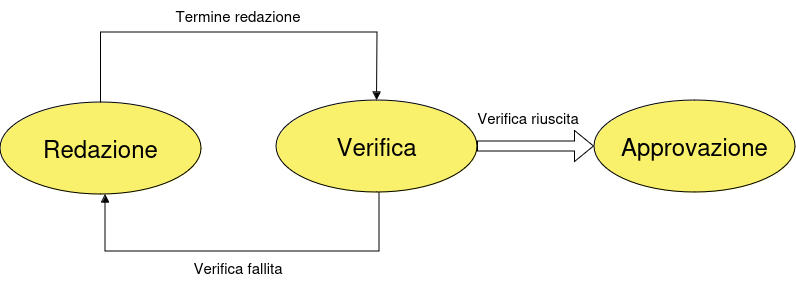
\includegraphics[width=0.6\textwidth]{Ciclo di vita della documentazione.png}
    \caption{Ciclo di vita della documentazione}
    \label{fig:ciclo_vita_documentazione}
\end{figure}


\subsubsection{Struttura dei documenti}
Ogni documento che verrà prodotto dovrà seguire una precisa struttura per garantire 
omogeneità e coesione.

\subsubsubsection{Numerazione di pagine}
La numerazione delle pagine del documento segue uno schema ben definito. Dalle pagine
iniziali e fino alla pagina precedente l’inizio del primo capitolo, viene utilizzata la numerazione
romana. Questa scelta mira a differenziare chiaramente la sezione introduttiva dal resto
del testo principale. Dopo questa fase preliminare, la numerazione prosegue con numeri
arabi, partendo da 1. Questo sistema offre una chiara progressione nel corpo principale del
lavoro. \\
Nel caso di appendici, la numerazione ritorna all’uso dei numeri romani, assegnando il numero 
I a ciascuna appendice.  Se ci sono più appendici, ogni volta che ne viene completata
una, si ricomincia la numerazione da I per la successiva. Questo approccio fornisce
un’organizzazione chiara e logica per le appendici, garantendo che ciascuna sia distintamente 
identificata. L’uso coerente di numeri romani e arabi in diverse sezioni del documento
contribuisce a una struttura ordinata e comprensibile per il lettore.

\subsubsubsection{Intestazione e piè di pagina}
In ciascuna pagina del documento, escludendo il frontespizio, sono presenti sia un’intestazione
che un piè di pagina. Nell’intestazione, sono inclusi i seguenti elementi:
\begin{itemize}
    \item Sul lato sinistro: il numero e il titolo del capitolo corrente;
    \item Sul lato destro: il logo del gruppo.
\end{itemize}
Nel piè di pagina, invece, sono indicati i seguenti dettagli:
\begin{itemize}
    \item Sul lato sinistro: il nome del file;
    \item Al centro: il numero della pagina attualmente in consultazione;
    \item Sul lato destro: il numero di versione del file.
\end{itemize}

\subsubsubsection{Frontespizio}
Il frontespizio, ovvero la prima pagina del documento,  strutturato nel seguente modo:
\begin{itemize}
    \item \textbf{Logo UniPD}: il logo universitario è posizionato in alto a sinistra;
    \item \textbf{Informazioni sul corso}: le informazioni relative al corso di Ingegneria del Software sono in alto a destra
    \item \textbf{Logo del gruppo}: il logo del gruppo è posizionato in alto a sinistra subito sotto al logo dell'Università;
    \item \textbf{Nome gruppo e recapito}: le informazioni sul gruppo \emph{SWEg Labs} sono posizionate in alto a destra, subito sotto alle info sul corso;
    \item \textbf{Titolo}: il titolo del documento è posizionato al centro della pagina, in grassetto;
    \item \textbf{Versione}: la versione del documento è posizionata al centro della pagina, appena sotto il titolo;
    \item \textbf{Tabella descrittiva}: posizionata centralmente sotto la versione del documento, riporta le seguenti informazioni:
    \begin{itemize}
        \item \textbf{Stato}: lo stato del documento nel suo ciclo di vita;
        \item \textbf{Redazione}: elenco dei membri del gruppo (nome e cognome) che hanno svolto la redazione del documento;
        \item \textbf{Verifica}: elenco dei membri del gruppo (nome e cognome) che hanno svolto la verifica del documento;
        \item \textbf{Approvazione}: elenco dei membri del gruppo (nome e cognome) che hanno svolto l’approvazione del documento;
        \item \textbf{Proprietario}: il proprietario del documento, nel nostro caso tutto il gruppo \emph{SWEg Labs};
        \item \textbf{Uso}: destinazione d’uso del documento (interno o esterno);
        \item \textbf{Destinatari}: destinatari del documento.
    \end{itemize}
\end{itemize}

\subsubsubsection{Registro delle modifiche}
Dopo la prima pagina si trova il registro delle modifiche. Tale registro va aggiornato ad ogni
modifica effettuata, specificando per ognuna:
\begin{itemize}
    \item \textbf{Versione}: la versione del documento in seguito alla modifica;
    \item \textbf{Data}: la data in cui è stata effettuata la modifica;
    \item \textbf{Descrizione}: una breve descrizione della modifica apportata;
    \item \textbf{Autore}: il nome e cognome dell’autore della modifica;
    \item \textbf{Verificatore}: il nome e cognome del verificatore della modifica, cioè
    colui che effettua la verifica del contenuto che è stato aggiungo, modificato o eliminato.
\end{itemize}

Le lettere di presentazione e i verbali, sia interni che esterni, non sono dotati del registro delle modifiche in quanto
in seguito alla prima redazione poi non sono soggetti a modifiche future.

\subsubsubsection{Indice}
Tutti i documenti (tranne le lettere di presentazione per ragione di brevità) devono contenere 
un indice, collocato nella pagina successiva al registro delle modifiche. L’indice è utile per 
agevolare la consultazione del documento, riportando per ogni titolo di sezione (e sottosezione) 
del contenuto effettivo del documento la sua pagina iniziale. Ciascuna delle pagine del contenuto 
è identificata da un numero progressivo, partendo da 1. In caso di sottosezioni si segue il formato:
\begin{center}
    \textbf{[numero sezione].[numero sottosezione]}
\end{center}
Lo stesso formato vale per qualsiasi livello di annidamento delle sottosezioni.

\subsubsubsection{Elenco delle figure}
Nella pagina successiva all’indice è presente l’elenco delle figure. Esso riporta, per ogni figura
che compare all’interno del documento, il suo titolo e la pagina in cui si trova. Come avviene
per le sezioni, ciascuna figura è identificata da un numero progressivo, partendo da 1.

\subsubsubsection{Elenco delle tabelle}
Nella pagina successiva a quelle dedicate all’elenco delle figure è presente l’elenco delle tabelle.
Esso riporta, per ogni tabella che compare all’interno del documento, il suo titolo e la pagina
in cui si trova. Come avviene per le sezioni e per l’elenco delle figure, ciascuna tabella è
identificata da un numero progressivo, partendo da 1.

\subsubsubsection{Contenuto}
Si tratta del contenuto effettivo del documento. Il contenuto deve essere suddiviso in sezioni
e sottosezioni, ciascuna con il suo titolo in grassetto e numerato secondo i criteri descritti in
precedenza.

\subsubsubsection{Verbali}
I verbali sono documenti che riportano le discussioni e le decisioni prese durante incontri.
I verbali devono contenere le seguenti sezioni:
\begin{itemize}
    \item \textbf{Informazioni generali}: contiene le informazioni riguardanti l’incontro, come la data, l’ora, il luogo e i partecipanti;
    \item \textbf{Ordine del giorno}: elenco degli argomenti che si era pianificato di trattare durante l’incontro;
    \item \textbf{Diario della riunione}: riassunto delle discussioni e delle azioni operate durante l’incontro;
    \item \textbf{Decisioni}: elenco delle decisioni prese durante l’incontro, ciascuna munita di codice identificativo per consentirne il tracciamento;
    \item \textbf{Todo}: elenco delle cose da fare emerse durante l'incontro, ciascuna collegata ad una o più decisioni. Ogni voce include un codice 
    identificativo per il tracciamento nel backlog, specifica la/e decisione/i di origine e il responsabile assegnato.
\end{itemize}


\subsubsection{Convenzioni}
In seguito vengono riportate tutte le convenzioni che i documenti devono rispettare.

\subsubsubsection{Nomi dei file}
Tutti i nomi dei file devono seguire la convenzione dello \emph{snake case}\textsubscript{\textit{\textbf{G}}}, 
cioè devono iniziare con una lettera minuscola e in caso di più parole ciascuna di esse deve essere separata tramite
il carattere di underscore ("\_"), tranne la data presente nei verbali, le cui parti devono essere separate da un trattino ("-"). Dopo il nome 
vero e proprio del file segue il numero della versione di quest’ultimo.

\subsubsubsection{Stile del testo}
Qui sono descritti tutti i diversi tipi di formattazione del testo usati nei documenti e i contesti
nei quali vengono impiegati:
\begin{itemize}
    \item \textbf{Grassetto}: viene utilizzato per evidenziare termini negli elenchi puntati e per i titoli
    delle sezioni;
    \item \textbf{Corsivo}: viene utilizzato per parole di particolare rilevanza all’interno del documento, 
    per indicare il nome del gruppo (\emph{SWEg Labs}), il nome dell’azienda \emph{proponente}\textsubscript{\textit{\textbf{G}}} 
    (\emph{AzzurroDigitale Srl}) e per le parole che si riferiscono al glossario (seguite da \textsubscript{\textit{\textbf{G}}});
    \item \textbf{Link}: i link sono i collegamenti ipertestuali, ovvero collegamenti a fonti esterne al
    documento. Essi sono mostrati sottolineati e in grassetto, mentre vengono evidenziati in giallo
    al momento del passaggio del cursore.
\end{itemize}

\subsubsubsection{Elenchi puntati}
Gli elenchi puntati sono utilizzati per gli elenchi oppure per esprimere concetti in modo più
diretto. Ciascuna voce di un elenco puntato è identificata da un simbolo, che varia a seconda
del livello di profondità in cui si trova. In particolare:
\begin{itemize}
    \item Un pallino per il primo livello;
    \begin{itemize}
        \item Un trattino per il secondo livello;
        \begin{itemize}
            \item Un asterisco per il terzo livello;
            \begin{itemize}
                \item Un punto per il quarto livello.
            \end{itemize}
        \end{itemize}
    \end{itemize}
\end{itemize}
Ogni voce inizia con la lettera maiuscola e termina con un punto e virgola (”;”), eccezione
fatta per l’ultima voce che termina con un punto (”.”).

\subsubsubsection{Formato delle date}
Per le date, viene adottato il seguente formato:
\begin{center}
    \textbf{DD/MM/YYYY}
\end{center}
dove:
\begin{itemize}
    \item \textbf{DD}: indica il giorno con 2 cifre;
    \item \textbf{MM}: indica il mese con 2 cifre;
    \item \textbf{YYYY}: indica l’anno con 4 cifre.
\end{itemize}

\subsubsubsection{Sigle}
Una lista di sigle presente all'interno dei documenti è la seguente:
\begin{itemize}
    \item \textbf{Ruoli}:
    \begin{itemize}
        \item \textbf{Re}: Responsabile di Progetto;
        \item \textbf{Am}: Amministratore di Progetto;
        \item \textbf{An}: Analista;
        \item \textbf{Pt}: Progettista;
        \item \textbf{Pr}: Programmatore;
        \item \textbf{Ve}: Verificatore.
    \end{itemize}
    \item \textbf{Revisioni di progetto}:
    \begin{itemize}
        \item \textbf{RTB}: \emph{Requirements and Technology Baseline}\textsubscript{\textit{\textbf{G}}};
        \item \textbf{PB}: \emph{Product Baseline}\textsubscript{\textit{\textbf{G}}}.
    \end{itemize}
\end{itemize}

\subsubsubsection{Tabelle}
Le tabelle di ogni documento devono rispettare le seguenti convenzioni:
\begin{itemize}
    \item Devono essere centrate orizzontalmente all’interno della pagina;
    \item Dopo ogni tabella segue una breve didascalia descrittiva accompagnata da un numero
    identificativo della stessa, incrementale e univoco all’interno del documento;
    \item Nelle celle che contengono solo uno 0 (zero), esso viene sostituito con un trattino per
    aumentarne la leggibilità.
\end{itemize}

\subsubsubsection{Immagini}
Ciascuna immagine, come le tabelle, deve essere centrata orizzontalmente all’interno della
pagina ed è seguita da una breve didascalia descrittiva comprensiva di un numero che le
identifica univocamente, incrementale all’interno del documento. Anche i grafici, 
\emph{diagrammi di Gantt}\textsubscript{\textit{\textbf{G}}} e \emph{diagrammi UML}\textsubscript{\textit{\textbf{G}}} 
sono inseriti nei documenti come immagini, pertanto seguono le stesse regole.


\subsubsection{Strumenti}
Per la redazione dei documenti, il gruppo \emph{SWEg Labs} ha scelto di utilizzare i seguenti strumenti:
\begin{itemize}
    \item \textbf{\emph{\LaTeX}}\textsubscript{\textit{\textbf{G}}}: per la redazione dei documenti il gruppo ha scelto il linguaggio \LaTeX. Si tratta
    di un linguaggio di markup basato su TeX per la produzione di documenti tecnici e scientifici di alta qualità;
    \item \textbf{\emph{Visual Studio Code}}\textsubscript{\textit{\textbf{G}}}: come editor di testo, il gruppo utilizza Visual Studio Code, 
    preferito per la sua leggerezza, versatilità e il supporto per estensioni personalizzabili;
    \item \textbf{\emph{GitHub}}\textsubscript{\textit{\textbf{G}}}: GitHub è utilizzato come piattaforma di versionamento e repository per la documentazione. 
    Consente una gestione collaborativa, permettendo il tracciamento delle modifiche e la revisione del testo in tempo reale;
    \item \textbf{\emph{draw.io}}\textsubscript{\textit{\textbf{G}}}: il team ha optato per Draw.io per disegnare i diagrammi UML necessari
    alla realizzazione del progetto didattico.
    \item \textbf{\emph{Fogli Google}}\textsubscript{\textit{\textbf{G}}}: i Fogli di calcolo di Google sono utilizzati dal team per creare e 
    aggiornare i grafici richiesti dal progetto.
\end{itemize}




\subsection{Gestione della configurazione}
\label{sec:gestione_configurazione}

\subsubsection{Scopo}
L’obiettivo di questa sezione è delineare l’approccio adottato dal gruppo \emph{SWEg Labs} nella 
gestione della configurazione, ossia la strategia scelta dal team per tenere traccia della
documentazione redatta e del codice sviluppato.

\subsubsection{Aspettative}
Per quanto riguarda la gestione della configurazione, il gruppo ha le seguenti aspettative:
\begin{itemize}
    \item Possibilità di tracciare tutte le modifiche apportate ai documenti o al codice;
    \item Possibilità di condivisione dei file tra i vari membri del gruppo;
    \item Possibilità di individuare e risolvere eventuali conflitti o errori;
    \item Possibilità di tornare ad una versione precedente.
\end{itemize}

\subsubsection{Descrizione}
L’obiettivo del processo di gestione della configurazione è garantire l’organizzazione e la
tracciabilità della documentazione e del codice, creando una storia per ogni file prodotto.
In particolare, si intende disporre i vari file all’interno di \emph{repository}\textsubscript{\textit{\textbf{G}}} 
facilmente accessibili e navigabili.


\subsubsection{Versionamento}

\subsubsubsection{Codice di versione}
Ad ogni modifica apportata ad un documento viene generata automaticamente una nuova
versione per quest’ultimo. Ogni versione è identificata dal suo codice, nel formato
\begin{center}
    \textbf{X.Y.Z}
\end{center}
dove:
\begin{itemize}
    \item \textbf{X}: rappresenta la versione dell’ultima approvazione da parte del responsabile;
    \item \textbf{Y}: rappresenta la versione dell’ultima approvazione generale da parte di un verificatore;
    \item \textbf{Z}: rappresenta la versione dell’ultima modifica, verificata da un verificatore.
\end{itemize}
Ogni approvazione comporta un incremento del numero di versione, che assume un peso
diverso a seconda della posizione della cifra incrementata: i cambiamenti più importanti
implicano un incremento della cifra più significativa.\\
Inoltre, un incremento ad una determinata cifra implica l’azzeramento di tutte le cifre alla
sua destra.

\subsubsubsection{Sistemi software utilizzati}
Per la gestione delle repository \emph{Git}\textsubscript{\textit{\textbf{G}}} si è deciso di utilizzare la 
piattaforma online \emph{GitHub}\textsubscript{\textit{\textbf{G}}}, in
quanto tutti i membri del gruppo hanno già familiarizzato in precedenza con questo sistema
software. Per quanto riguarda la gestione del \emph{backlog}\textsubscript{\textit{\textbf{G}}}, si è deciso di utilizzare
il servizio offerto da \emph{Jira}\textsubscript{\textit{\textbf{G}}}, dal momento che permette di usare strumenti avanzati per la
pianificazione, tracciamento e gestione dell’assegnazione delle varie attività.


\subsubsection{Struttura delle repository}
Con l’intento di organizzare al meglio il lavoro, si è optato per la creazione di due distinte 
repository pubbliche, al fine di mantenere separati i documenti organizzativi e il software:
\begin{itemize}
    \item \textbf{Documentazione}: per il versionamento della documentazione;
    \item \textbf{BuddyBot}: per il versionamento del codice.
\end{itemize}

\subsubsubsection{Documentazione}
\label{sec:repo_documentazione}
All’interno di questa repository sono presenti le cartelle relative alle principali \emph{milestone}\textsubscript{\textit{\textbf{G}}}
del progetto, contenenti le rispettive \emph{baseline}\textsubscript{\textit{\textbf{G}}}:
\begin{itemize}
    \item \textbf{Candidatura}:  in questa cartella sono presenti i documenti prodotti per la candidatura
    d’appalto per il Capitolato C9. Il contenuto di questa cartella è il seguente:
    \begin{itemize}
        \item \textbf{Lettera di presentazione (v1.0.0)}: documento con cui il gruppo \emph{SWEg Labs} si
        candida formalmente per la realizzazione del progetto commissionato;
        \item \textbf{Preventivo dei costi e degli impegni orari (v1.0.0)}: documento che contiene 
        l’impegno orario per ciascun membro del gruppo, il costo totale preventivato per la
        realizzazione del progetto e la scadenza di consegna del prodotto software. Tali
        conclusioni sono tratte da alcune considerazioni preliminari sui ruoli che i membri
        del gruppo dovranno svolgere e da previa consultazione con il proponente \emph{AzzurroDigitale}\textsubscript{\textit{\textbf{G}}};
        \item \textbf{Valutazione dei Capitolati (v1.0.0)}: documento in cui il gruppo valuta 
        le criticità riscontrate per ogni capitolato d’appalto e motiva la scelta del
        capitolato selezionato;
        \item \textbf{Verbali}: cartella contenente tutti i verbali interni ed esterni (raccolti in apposite sottocartelle)
        relativi al periodo di candidatura;
    \end{itemize}
    \item \textbf{RTB}: in questa cartella sono presenti i documenti prodotti per la candidatura alla \emph{RTB}\textsubscript{\textit{\textbf{G}}}.
    Il contenuto è composto da:
    \begin{itemize}
        \item \bulhref{https://sweg-labs.github.io/Documentazione/output/RTB/lettera_presentazione.pdf}{Lettera di Presentazione};
        \item \textbf{Documentazione esterna}: sono contenuti i seguenti documenti:
        \begin{itemize}
            \item \bulhref{https://sweg-labs.github.io/Documentazione/output/RTB/Documentazione\%20esterna/analisi_requisiti_v1.0.0.pdf}{Analisi dei Requisiti (v1.0.0)};
            \item \bulhref{https://sweg-labs.github.io/Documentazione/output/RTB/Documentazione\%20esterna/piano_progetto_v1.0.0.pdf}{Piano di Progetto (v1.0.0)};
            \item \bulhref{https://sweg-labs.github.io/Documentazione/output/RTB/Documentazione\%20esterna/piano_qualifica_v1.0.0.pdf}{Piano di Qualifica(v1.0.0)};
            \item \textbf{Verbali esterni}: cartella che raccoglie tutti i verbali esterni relativi al periodo RTB.
        \end{itemize}
        \item \textbf{Documentazione interna}: al suo interno sono contenuti:
        \begin{itemize}
            \item \bulhref{https://sweg-labs.github.io/Documentazione/output/RTB/Documentazione\%20interna/norme_progetto_v1.0.0.pdf}{Norme di Progetto (v1.0.0)};
            \item \bulhref{https://sweg-labs.github.io/Documentazione/output/RTB/Documentazione\%20interna/glossario_v1.0.0.pdf}{Glossario};
            \item \textbf{Verbali interni}: cartella che raccoglie tutti i verbali interni relativi al periodo RTB.
        \end{itemize}
    \end{itemize}
    \item \textbf{PB}: in questa cartella sono presenti i documenti prodotti per la candidatura alla \emph{PB}\textsubscript{\textit{\textbf{G}}}.
    Il contenuto è composto da:
    \begin{itemize}
        \item \bulhref{https://sweg-labs.github.io/Documentazione/output/PB/lettera_presentazione.pdf}{Lettera di Presentazione};
        \item \textbf{Documentazione esterna}: sono contenuti i seguenti documenti:
        \begin{itemize}
            \item \bulhref{https://sweg-labs.github.io/Documentazione/output/PB/Documentazione\%20esterna/analisi_requisiti_v2.0.0.pdf}{Analisi dei Requisiti (v2.0.0)};
            \item \bulhref{https://sweg-labs.github.io/Documentazione/output/PB/Documentazione\%20esterna/piano_progetto_v2.0.0.pdf}{Piano di Progetto (v2.0.0)};
            \item \bulhref{https://sweg-labs.github.io/Documentazione/output/PB/Documentazione\%20esterna/piano_qualifica_v2.0.0.pdf}{Piano di Qualifica(v2.0.0)};
            \item \bulhref{https://sweg-labs.github.io/Documentazione/output/PB/Documentazione\%20esterna/specifica_tecnica_v1.0.0.pdf}{Specifica Tecnica (v1.0.0)};
            \item \bulhref{https://sweg-labs.github.io/Documentazione/output/PB/Documentazione\%20esterna/manuale_utente_v1.0.0.pdf}{Manuale Utente (v1.0.0)};
            \item \textbf{Verbali esterni}: cartella che raccoglie tutti i verbali esterni relativi al periodo PB.
        \end{itemize}
        \item \textbf{Documentazione interna}: al suo interno sono contenuti:
        \begin{itemize}
            \item \bulhref{https://sweg-labs.github.io/Documentazione/output/PB/Documentazione\%20interna/norme_progetto_v2.0.0.pdf}{Norme di Progetto (v2.0.0)};
            \item \bulhref{https://sweg-labs.github.io/Documentazione/output/PB/Documentazione\%20interna/glossario_v2.0.0.pdf}{Glossario};
            \item \textbf{Verbali interni}: cartella che raccoglie tutti i verbali interni relativi al periodo PB.
        \end{itemize}
    \end{itemize}
\end{itemize}

\subsubsubsection{BuddyBot}
\label{sec:repo_buddybot}
Questa repository contiene il codice sorgente relativo al \emph{Minimum Viable Product}\textsubscript{\textit{\textbf{G}}} del progetto e le
istruzioni per scaricarlo e testarlo in locale (\emph{README.md}).
Inoltre, è presente un file chiamato prompt\_engineering.txt dove sono riportati tutti i tentativi operati 
per raggiungere un miglioramento dell'efficacia informativa delle risposte di BuddyBot, 
tra cui varie domande poste al chatbot e le corrispondenti risposte ottenute nel corso del tempo.

\subsubsubsection{Gestione delle modifiche}
Una buona suddivisione del lavoro tra i diversi documenti da redigere e le varie \emph{feature}\textsubscript{\textit{\textbf{G}}}
da sviluppare contribuisce significativamente a ridurre i conflitti. L’obiettivo è mantenere 
il \emph{branch}\textsubscript{\textit{\textbf{G}}} principale (\emph{main}) privo di errori, rendendolo inaccessibile a qualsiasi membro 
del gruppo fino all’approvazione del Responsabile di Progetto. Solo in seguito di tale
approvazione è consentito effettuare il \emph{merge}\textsubscript{\textit{\textbf{G}}} di uno dei rami minori nel \emph{main}.


\subsection{Gestione della Qualità}
\label{sec:gestione della qualità}

\subsubsection{Scopo}
Questa sezione ha l'obbiettivo di descrivere le modalità con cui il gruppo intende misurare la qualità dei processi e del prodotto finale, al fine di soddisfare le aspettative del proponente.

\subsubsection{Descrizione}
Il processo di gestione della qualità stabilisce le norme e gli strumenti per misurare della qualità dei processi e del prodotto finale. Sono specificati gli obbiettivi prefissati, i metodi per raggiungerli e per verificarne il compimento.

\subsubsection{Aspettative}
\begin{itemize}
    \item Soddisfare i requisiti di qualità richiesti dal proponente;
    \item Migliorare la qualità dei processi svolti dal gruppo;
    \item Valutare lo stato di avanzamento del progetto.
\end{itemize}

\subsubsection{Piano di Qualifica}
Per stabilire gli obbiettivi di questo processo utilizziamo il Piano di Qualifica. Ossia un documento contenente:
\begin{itemize}
    \item Gli obbiettivi qualitativi da raggiungere;
    \item Le definizioni e descrizioni delle metriche utilizzate per la misurazione della qualità dei processi, del prodotto, della documentazione e dei software utilizzati;
    \item La descrizione dei test da svolgere e le relative norme da seguire;
    \item Lo stato attuale della qualità del progetto, misurato tramite le metriche descritte.
\end{itemize}

\subsubsection{Strumenti}
Gli strumenti utilizzati per la gestione della qualità sono le metriche.
Queste sono le norme che regolano le metriche adottate, le quali rappresentano ognuna un conseguente obiettivo prefissato.
Le metriche adottate sono presentate e descritte nel documento piano di qualifica, ognuna con i seguenti parametri:
\begin{itemize}
    \item \textbf{Nome}: il nome della metrica
    \item \textbf{Codice}: ogni metrica ha un codice identificativo formato da:
    \begin{center}
        M[Tipologia][Id numerico]
    \end{center}
    dove
    \begin{itemize}
        \item \textbf{Tipologia} può essere:
        \begin{itemize}
            \item \textbf{PC} per processo;
            \item \textbf{PD} per prodotto.
        \end{itemize}
        \item \textbf{Id numerico} indica un numero univoco incrementale separato per le due tipologie.
    \end{itemize}
    \item \textbf{Processo}: indica a che processo fa riferimento la metrica;
    \item \textbf{Formula}: come la metrica viene matematicamente calcolata (opzionale);
    \item \textbf{Descrizione}: spiegazione di cosa rappresenta la metrica e di come valutarla e interpretarla;
    \item \textbf{Valore di accettabilità}: indica il valore della metrica considerato accettabile;
    \item \textbf{Valore di preferibilità}: indica il valore ideale che dovrebbe essere assunto.
\end{itemize}


\subsection{Verifica}
\label{sec:verifica}

\subsubsection{Scopo}
Questa sezione si propone di illustrare come il gruppo ha pianificato e implementato il processo di \emph{verifica}\textsubscript{\textit{\textbf{G}}}, finalizzato a valutare il prodotto software. Tale processo è essenziale per garantire che il software soddisfi i requisiti definiti e rispetti le aspettative. 

\subsubsection{Aspettative}
\begin{itemize}
    \item Garantire l'ottenimento del prodotto finale in linea con le aspettative;
    \item Individuare tempestivamente eventuali errori, riducendo sprechi di risorse e tempo;
    \item Consentire al gruppo di progredire nello sviluppo in maniera più sicura e accurata.
\end{itemize}

\subsubsection{Descrizione}
Il processo di \emph{verifica}\textsubscript{\textit{\textbf{G}}} si basa su \emph{test}\textsubscript{\textit{\textbf{G}}} e analisi per individuare e correggere eventuali errori emersi durante lo sviluppo del software o la redazione della documentazione, assicurando la conformità ai requisiti. Per una verifica efficace, è fondamentale applicare procedure definite, criteri affidabili e una sequenza di fasi che preparino al passaggio successivo, ossia la validazione. Di seguito sono illustrate le principali attività svolte in questo processo.

\subsubsection{\emph{Analisi statica}\textsubscript{\textit{\textbf{G}}}}
L’\emph{analisi statica} prende il nome dal fatto che non richiede l’esecuzione del codice e si presta anche all’applicazione sulla documentazione. Questa attività consiste in una revisione dettagliata del codice e dei documenti per assicurarsi che rispettino i vincoli stabiliti, siano privi di difetti e soddisfino le caratteristiche richieste
Il successo di questa analisi dipende in modo significativo dalla competenza e dall’attenzione dei verificatori coinvolti.

\subsubsection{\emph{Analisi dinamica}\textsubscript{\textit{\textbf{G}}}}
L'\emph{analisi dinamica} comprende tecniche che richiedono l'esecuzione del codice da verificare, rendendola applicabile esclusivamente al software, e non alla documentazione. 
Questa attività prevede l'esecuzione di \emph{test}\textsubscript{\textit{G}} per verificare il corretto funzionamento del software e identificare eventuali discrepanze tra i risultati attesi e quelli effettivi. Questo processo deve essere automatizzato e ripetibile. 
Per garantire l'efficacia dei test, ciascuno di essi deve essere deterministico, cioè, dati gli stessi input, deve produrre sempre lo stesso output. 
Inoltre, ogni test deve avere parametri ben definiti, tra cui:
\begin{itemize}
    \item descrizione dei parametri di input;
    \item descrizione dell'output;
    \item comportamento atteso del software;
    \item condizioni di esecuzione del test.
\end{itemize}
Al fine di agevolare l’automazione dei test, saranno utilizzati i seguenti strumenti:
\begin{itemize}
    \item \textbf{Driver:} una componente che fornisce l’ambiente di esecuzione necessario per testare un componente del prodotto software. Un driver è progettato per “attivare” il componente da testare e fornirgli i dati di input necessari;
    \item \textbf{Stub:} una componente passiva che simula il comportamento di alcune parti mancanti o non ancora implementate nell’applicazione. Questo consente di testare in anticipo le parti del software che dipendono da altre parti non ancora disponibili;
    \item \textbf{Logger:} uno strumento che registra i risultati ottenuti durante l’esecuzione del test, consentendo un’analisi accurata dei dati prodotti.
\end{itemize}

\subsubsection{Test di sistema}
I \emph{Test di sistema}\textsubscript{\textit{\textbf{G}}} hanno l’obiettivo di misurare la copertura dei requisiti specificati nel
capitolato d’appalto. Essi sono definiti durante l’\emph{Analisi dei Requisiti} e vengono svolti dopo
i \emph{test di integrazione}, dunque quando tutte le componenti del sistema software sono state
integrate. Questo tipo di test è svolto anche durante il processo di validazione.

\subsubsection{Test di accettazione}
I \emph{Test di accettazione}\textsubscript{\textit{\textbf{G}}} servono per dimostrare che i requisiti individuati sono stati
soddisfatti. Questo tipo di test deve essere svolto obbligatoriamente alla presenza del \emph{committente}.

\subsubsection{Codici relativi ai test}
Il gruppo ha deciso di classificare i \emph{test} che andranno svolti nell’attività di verifica associando un codice identificativo a ciascuno di essi nel formato
\begin{center}
    \textbf{T[tipo][codice]}
\end{center}T[tipo][codice]
dove:
\begin{itemize}
    \item \textbf{[tipo]} rappresenta il tipo di test, in particolare:
    \begin{itemize}
        \item S per i test di sistema;
        \item A per i test di accettazione.
    \end{itemize}
    \item \textbf{[codice]} è un numero progressivo associato al test all’interno del suo tipo.
\end{itemize}

%Ancora da capire se serve: Se il test in questione ha un padre, si segue il formato [codice padre].[codice figlio]
%dove [codice figlio] è un numero progressivo che identifica univocamente un test figlio del test con codice pari a [codice padre].

\subsubsection{Stato dei test}
Ad ogni test verrà associato uno stato che ne rappresenterà l’esito.
Lo stato può essere:
\begin{itemize}
    \item N-I: il test non è ancora stato implementato;
    \item Superato: il test riporta esito positivo;
    \item Non superato: il test riporta esito negativo.
\end{itemize}

\subsection{Validazione}
\label{sec:validazione}
\subsubsection{Scopo}
Questa sezione contiene le norme atte a regolare il processo di validazione, al fine di garantirne l'efficacia. Il processo di validazione permette di confermare l'effettivo conseguimento delle aspettative specificate dal proponente.
\subsubsection{Aspettative}
Tramite il processo di validazione il gruppo intende assicurarsi la conformità del prodotto software rispetto ai requisiti specificati nel documento di Analisi dei Requisiti.
\subsubsection{Descrizione}
La validazione si articola in più attività:
\begin{itemize}
    \item \textbf{Istanziazione delle procedure}: vengono stabilite le procedure e le strategie da attuare per garantire una validazione efficace;
    \item \textbf{Istanziazione tei test di accettazione}: un test di accettazione consiste in una serie di operazioni eseguite sul prodotto software finale che rispondono positivamente solo se il software soddisfa tutti i requisiti specificati, garantendo che sia conforme alle aspettative del proponente. Tali test devono essere riportati nel documento \emph{Piano di qualifica};
    \item \textbf{Collaudo}: i test di accettazione vengono effettuati sul prodotto software in presenza del proponente, ma non prima di aver svolto con successo i test di sistema in un ambiente identico a quello di installazione.
\end{itemize}

\newpage
% Intestazione
\fancyhead[L]{4 \hspace{0.2cm} Processi organizzativi} % Testo a sinistra


\section{Processi organizzativi}

\dots
\newpage
% Intestazione
\fancyhead[L]{A \hspace{0.2cm} Standard ISO/IEC 12207} % Testo a sinistra

\pagenumbering{roman} % Numerazione romana per l'appendice

\appendix % Cambia la numerazione delle sezioni da numeri a lettere


\section{Standard ISO/IEC 12207}

L'\emph{ISO/IEC/IEEE 12207}\textsubscript{\textit{\textbf{G}}} definisce un framework completo per il ciclo di vita del software, identificando processi, attività e compiti necessari per sviluppare, gestire e mantenere software in modo sistematico. Implementare questo standard permette di mantenere un alto livello di qualità, tracciabilità e coerenza nei processi di sviluppo software. Fornisce un quadro di riferimento robusto per gestire i progetti, favorendo il miglioramento continuo e il rispetto delle tempistiche e dei requisiti iniziali.\\
Lo standard si articola in tre principali categorie di processi:
\begin{itemize}
    \item Processi primari
    \item Processi di supporto
    \item Processi organizzativi
\end{itemize}

\subsection{I processi primari}
I processi primari comprendono quelli necessari alla gestione e allo sviluppo del software, includendo sia la gestione del progetto sia il supporto tecnico.
\begin{itemize}
    \item \textbf{Processo di acquisizione}: Coinvolge tutte le attività di acquisizione del software o di servizi legati al software, come la definizione dei requisiti dell'acquirente, la selezione del fornitore, la gestione del contratto e il monitoraggio del progresso.
    \item \textbf{Processo di fornitura}: Descrive le attività del fornitore per sviluppare, modificare e consegnare il software in base alle specifiche di contratto. Include la pianificazione, lo sviluppo, la consegna e la gestione del software.
    \item \textbf{Processo di sviluppo}: Definisce le attività per creare o modificare il software. Le fasi principali sono:
    \begin{itemize}
        \item \textbf{Analisi dei requisiti}: Identificazione delle specifiche funzionali e non funzionali.
        \item \textbf{Progettazione del sistema e del software}: Progettazione dell'architettura e della struttura del software.
        \item \textbf{Implementazione}: Programmazione del codice sorgente.
        \item \textbf{Integrazione}: Assemblaggio delle diverse parti del software.
        \item \textbf{Testing}: Verifica del software per assicurare che rispetti i requisiti definiti.
        \item \textbf{Installazione e accettazione}: Rilascio del software e conferma della sua aderenza ai requisiti.
    \end{itemize}
    \item \textbf{Processo di gestione operativa}: Si occupa delle attività di gestione del software nel suo ambiente di produzione, incluse la manutenzione, il supporto utente, l'operatività continua e il monitoraggio delle performance.
    \item \textbf{Processo di manutenzione}: Comprende tutte le attività per correggere, migliorare o adattare il software dopo il rilascio, al fine di mantenerne o aumentarne l'efficienza e la rilevanza.
\end{itemize}

\subsection{I processi di supporto}
Questi processi assistono i processi primari e garantiscono che il software sia conforme agli standard di qualità.
\begin{itemize}
    \item \textbf{Processo di documentazione}: Definisce la creazione, la gestione e la manutenzione della documentazione di progetto.
    \item \textbf{Processo di configurazione}: Gestisce le versioni del software, tenendo traccia delle modifiche e assicurando che ogni versione sia stabile e rintracciabile.
    \item \textbf{Processo di verifica}: Garantisce che ogni fase dello sviluppo rispetti i requisiti iniziali attraverso attività di verifica e review, che coinvolgono sia il codice che la documentazione.
    \item \textbf{Processo di validazione}: Assicura che il software finale soddisfi le esigenze dell'utente, attraverso attività di testing e collaudo in condizioni reali.
    \item \textbf{Processo di qualità}: Definisce le attività di controllo qualità per monitorare la conformità agli standard e migliorare continuamente i processi di sviluppo.
    \item \textbf{Processo di revisione e audit}: Prevede revisioni periodiche e audit di progetto per identificare eventuali problemi o non conformità rispetto agli standard definiti.
\end{itemize}

\subsection{I processi organizzativi}
I processi organizzativi mirano a sostenere e migliorare i processi aziendali nel loro insieme, creando un ambiente di supporto che faciliti l'attività dei team.
\begin{itemize}
    \item \textbf{Processo di gestione}: Include tutte le attività di pianificazione, coordinamento e monitoraggio del progetto, come l'assegnazione delle risorse, la definizione del budget e la gestione del rischio.
    \item \textbf{Processo di miglioramento}: Riguarda le attività di analisi e ottimizzazione dei processi, come la raccolta di feedback, l'identificazione delle aree di miglioramento e la messa in atto di strategie di ottimizzazione.
    \item \textbf{Processo di formazione}: Definisce la formazione continua per il personale, migliorando le competenze tecniche e manageriali necessarie a svolgere i vari processi.
    \item \textbf{Processo di gestione delle risorse umane}: Include le attività di selezione, valutazione e gestione delle risorse umane impiegate nei vari processi.
\end{itemize}

\dots
\newpage
\input{contenuti/standard_qualità_iso-iec_9126.tex}
\newpage
\input{contenuti/metriche_qualità.tex}

\end{document}
